\documentclass{article}
\usepackage[utf8]{inputenc}
\usepackage{graphicx}
\usepackage[margin=0.5in]{geometry}
\title{Stat490 Homework}
\author{ANDY LI}
\date{February 2023}

\begin{document}

\maketitle
Fixed Effects Model:
\\Let $$SSTr = \sigma^2 + \sum_{i=1}^{k} \sum_{j=1}^{n_i} (Y_{ij} - \bar{Y_i})^2$$
\\
such that k is the number of levels of the factor, $n_i$ is the number of observations in the ith level and $Y_{ij}$ is the jth observation at the ith level.
\\
Let $\alpha_i = \frac{1}{n_i} \sum_{j=1}^{n_i} Y_{ij}$

Then, $$MSTr = SSTr - \sum_{i=1}^{k} n_i (\alpha_i - \bar{Y})^2$$

$$E(MSTr) = E(SSTr) - \sum_{i=1}^{k} n_i E[(\alpha_i - \bar{Y})^2]$$

$$E(MSTr) = \sigma^2 + \sum_{i=1}^{k} \sum_{j=1}^{n_i} E[(Y_{ij} - \bar{Y_i})^2] \Rightarrow 
E(MSTr) = \sigma^2 + \frac{1}{k-1}\sum_{i} \alpha_i^2$$

\\Random Effects Model:
$E(MSTr) = \frac{1}{a-1}E[\sum_{i=1}^a \frac{y_{i.}^2}{n}-\frac{y_{..}^2}{N}]$
$$= \frac{1}{a-1} E[\frac{1}{n} \sum_{i=1}^{a}(\sum_{j=1}^{n} \mu + \gamma_i + \epsilon_{ij})^2 - \frac{1}{N}(\sum_{i=1}^a \sum_{j=1}^n \mu + \gamma_i + \epsilon_{ij})^2]$$
$$\Rightarrow \frac{1}{a-1}(N\mu^2 + N\sigma_{\gamma}^2 + a\sigma^2 - N\mu^2 -n\sigma_{\gamma}^2-\sigma^2)$$
$$= \sigma^2 + n\sigma_{\gamma}^2$$

\section*{3.7}
$Df_{factor} = 4$       
\\$SS_{factor} = 1174.24 - 186.53 = 987.71$
\\$MSE = \frac{186.53}{25} = 7.4612$
\\$MSB = \frac{987.71}{4} = 246.93
\\F = \frac{MSB}{MSE} = \frac{246.93}{7.4612} = 33.0952$
\\From F table, $p = 1.185e-9$

\section*{3.9}
a)
\\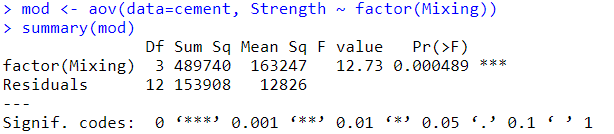
\includegraphics{3.9a.PNG}
\\b) 
\\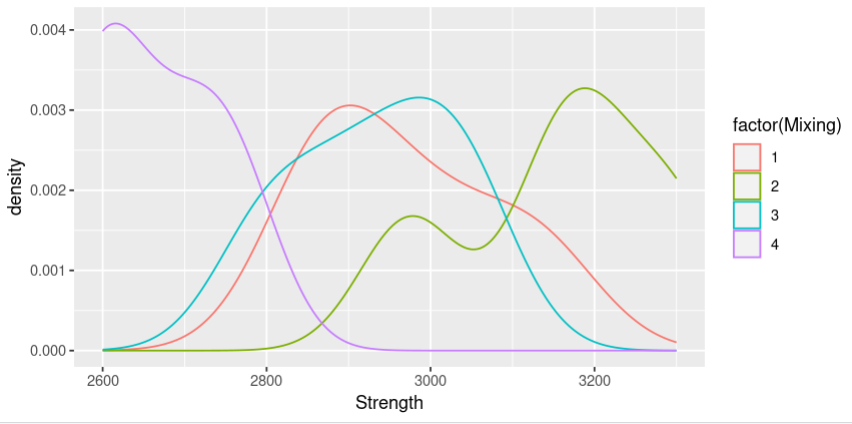
\includegraphics{3.9b.PNG}
\\Mixtures 1 and 3 have similar means around 2950. Mixture 2 has a higher mean around 3150, and mixture 4 has a lower mean around 2650.
\\
\\c)
\\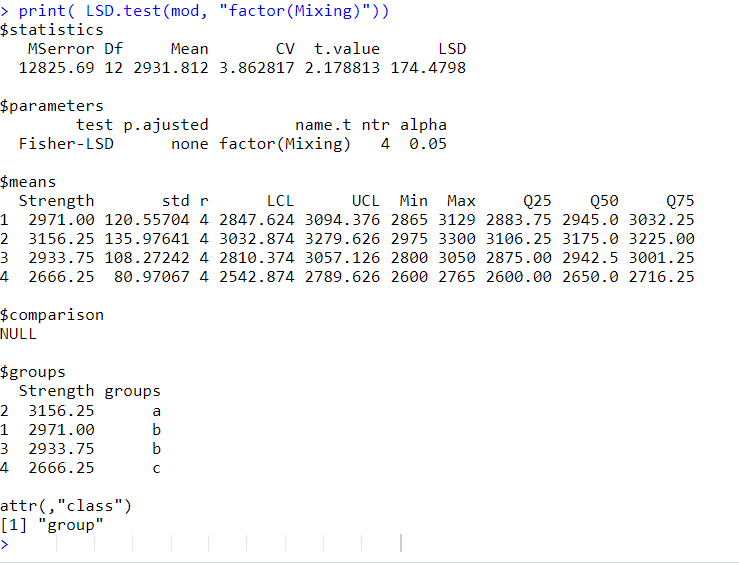
\includegraphics{3.9c.PNG}
\newpage
d)
\\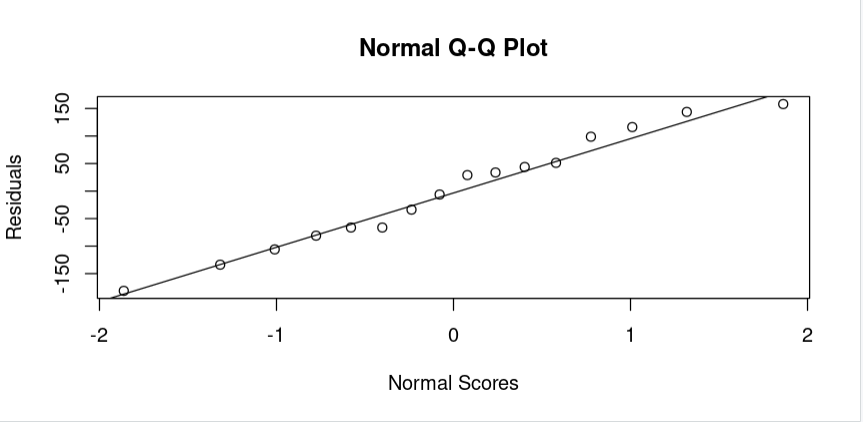
\includegraphics{9.3d.PNG}
\\According to the Normal Q-Q plot, the standardized residuals show that the sample is approximately normal. Therefore the normality assumption is valid.
\\
\\e)
\\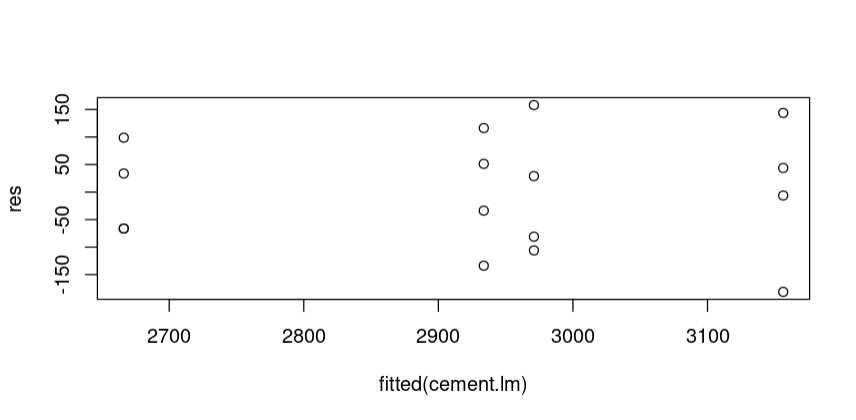
\includegraphics{9.3e.PNG}
\\The residuals for each of the mixtures seem equally spread further confirming the validity of the normality assumption.
\newpage
\\f) 
\\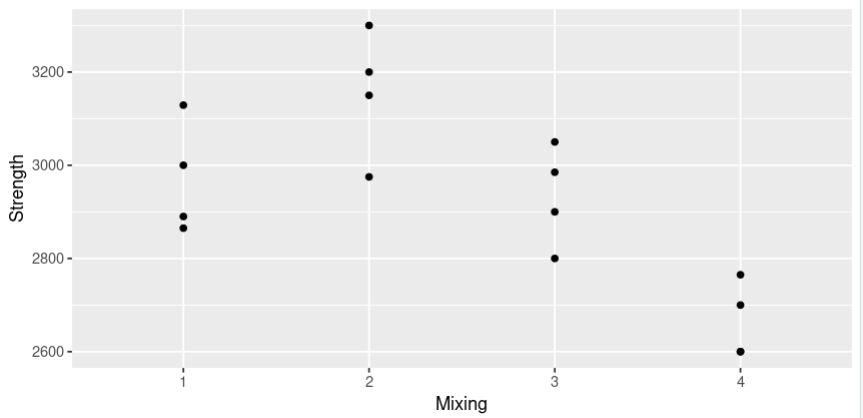
\includegraphics{3.9f.PNG}

\section*{3.10}
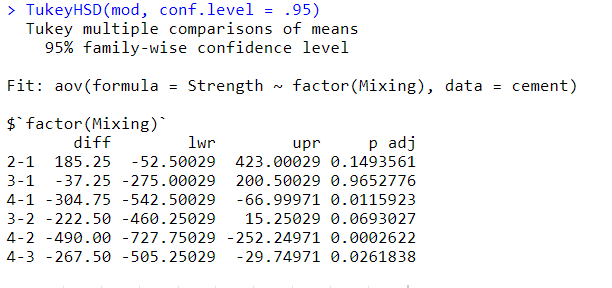
\includegraphics{3.10a.PNG}
\\Fisher LSD uses the t distribution and only finds the minimum difference. On the other hand, Tukey's HSD finds all the possible pair combinations and finds their differences.

\section*{3.13}
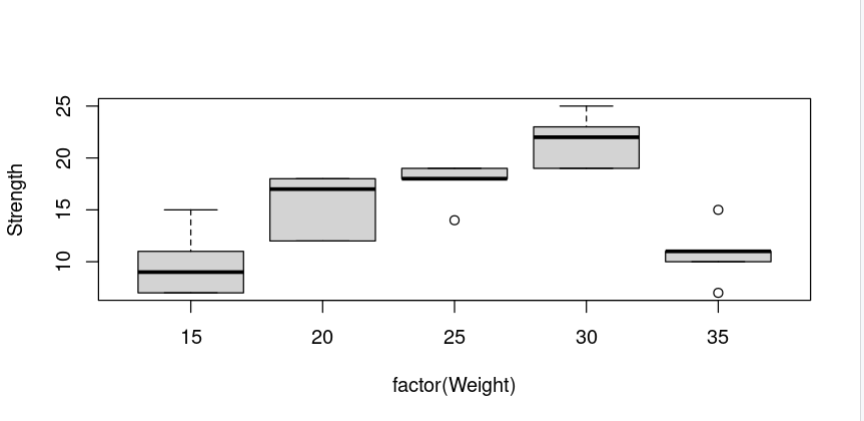
\includegraphics{13.10bp.PNG}
\\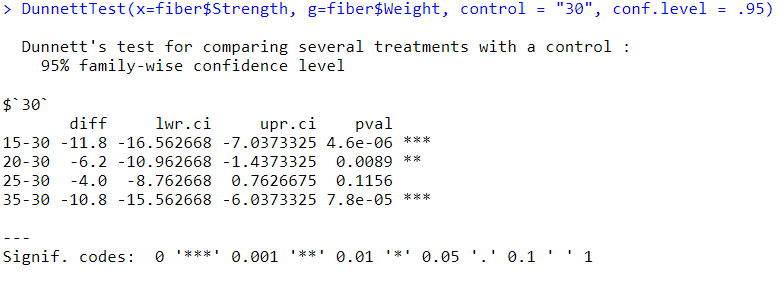
\includegraphics{13.13a.PNG}
\newpage
\section*{3.29}
a)
\\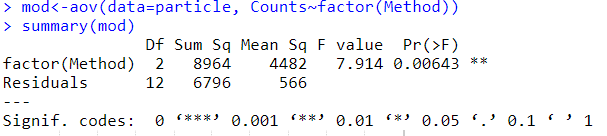
\includegraphics{13.29a.PNG}
\\From the ANOVA table, we see that the p value is small. Therefore, we can reject the null hypothesis that all methods produce the same count. In other words, all the methods do not have the same effect on particle count.
\\
\\b) 
\\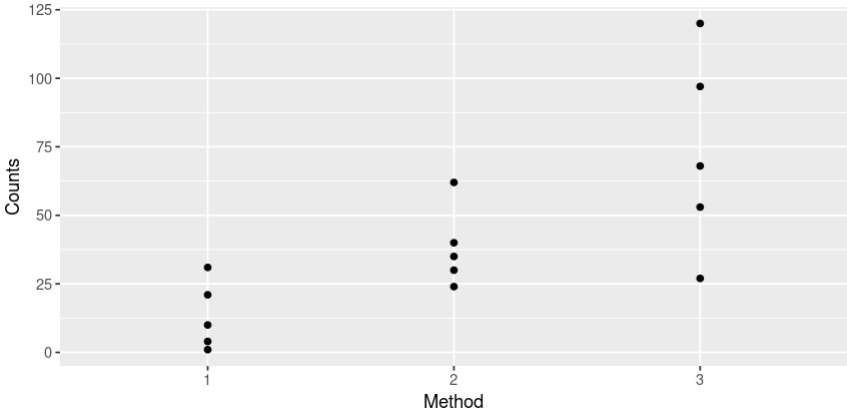
\includegraphics{3.29bsp.PNG}
\\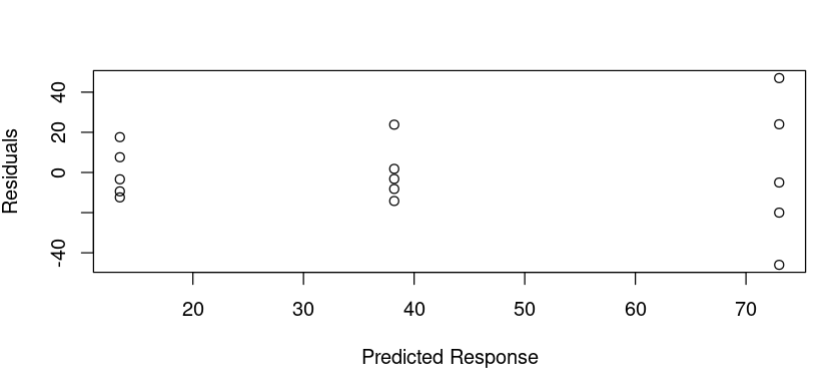
\includegraphics{3.29brp.PNG}
\\For Method 2, the residual plot shows an uneven spread of points. This hints at the fact that the data is not normal, thus the normality assumption may not be valid.
\\
\section*{3.34}
Number of levels = 6
\\Total sample size $N = 6 * 5 = 30$
$SSTr = 750.50$, $SST = 900.25$
\\a) Estimate of error variance $$\sigma^2 = \frac{SSE}{30-6} = \frac{900.25-750.50}{24} = 6.2396$$
\\
\\b) Coefficient of determination: $$r^2 = 1 - \frac{SSE}{SST} = 1 - \frac{149.75}{900.25} = .8337$$
$83.37\%$ of the variability in the response variable is explained by the treatment effect.
\\
\section*{3.40}
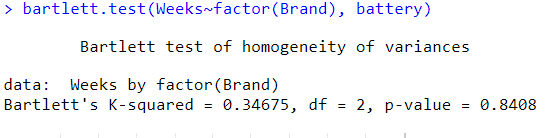
\includegraphics{3.40.PNG}
\\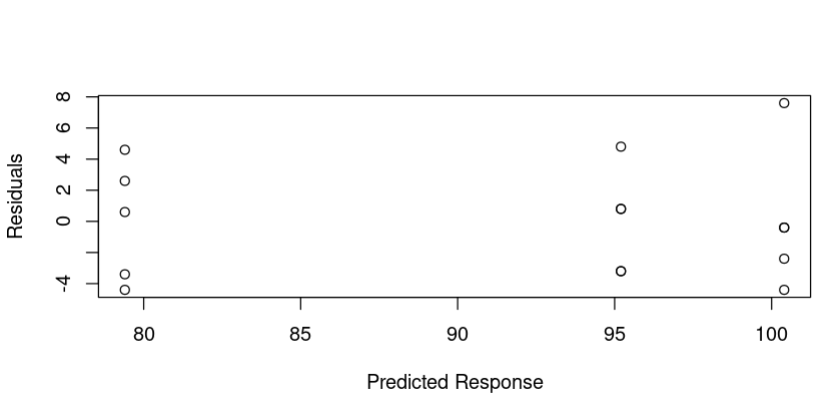
\includegraphics{3.40sp.PNG}
\\From Bartlett's test, we get a high p-value indicating that we fail to reject the null which says that all the variances are the same. In the residual plot, we see that the brands all have similar residuals which does not contradict the equal variance claim.
\newpage
\section*{3.46}
a) Error variance 36: $$\phi^2 = \frac{100n}{4(36)} = 0.6944n \Rightarrow \phi = \sqrt{0.6944n}$$
\\Hence, n = 7 from the OC curves.
\\
\\b) Error variance 49: $$\phi^2 = \frac{100n}{4(49)} = 0.5102n \Rightarrow \phi = \sqrt{0.5102n}$$
\\Hence, n = 9 from the OC curves.
\\
\\c) In order to keep the same $1-\beta$ while increasing variability, the sample size must also increase.
\\
\\d) Have an interval of possible variances which will provide an interval of sample sizes.
\\
\section*{3.53}
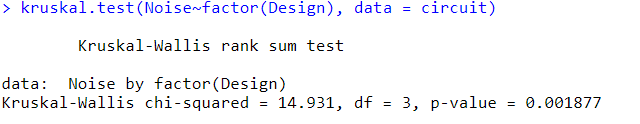
\includegraphics{3.53.PNG}
\\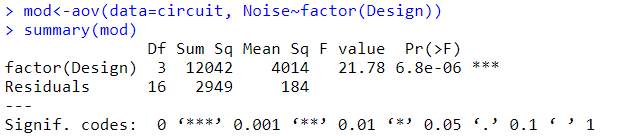
\includegraphics{3.53aov.PNG}
\\We see that the p value for Kruskal-Wallis is larger than ANOVA. However, both p values are small enough to reject the null hypotheses.
\end{document}
